Das ALICE Experiment wurde speziell zur Untersuchung des Quark-Gluonen-Plasmas konzipiert und gebaut.
%Um die Anspr\"uche daf\"ur besonders gut erf\"ullen zu k\"onnen besteht das ALICE Experiment aus einer Vielzahl unterschiedlicher Detektoren.
\begin{figure}[thp]
\centering
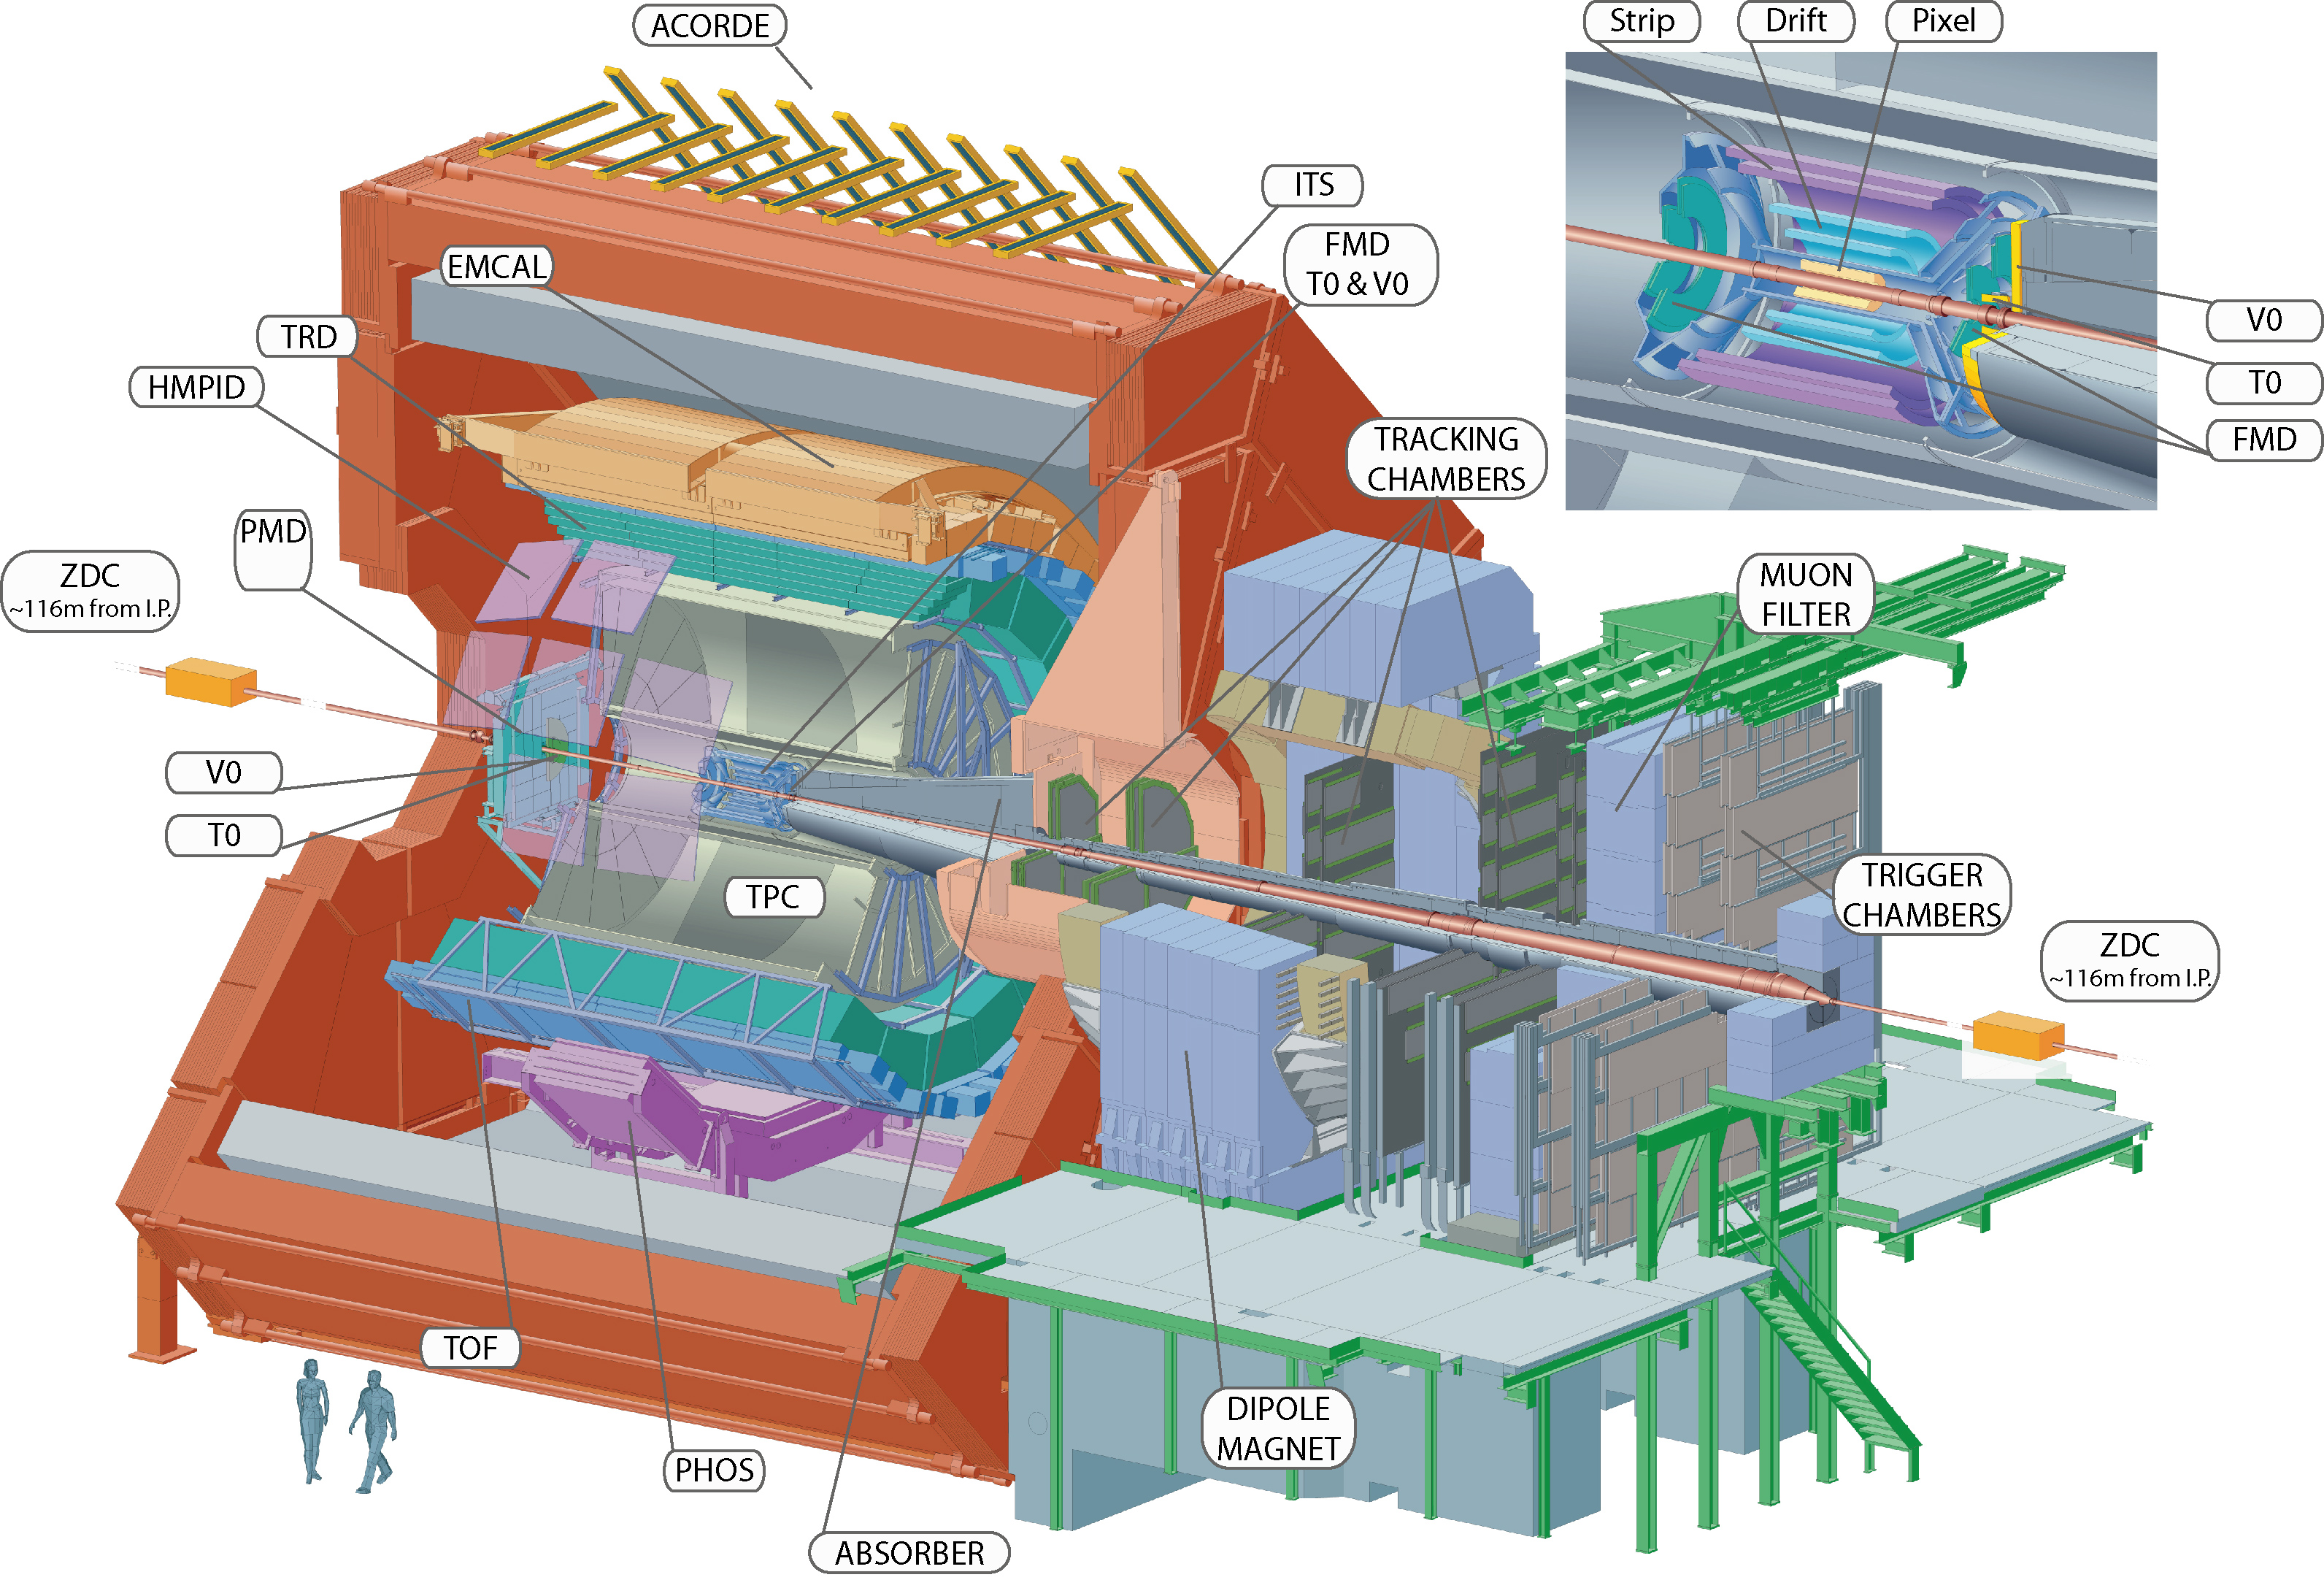
\includegraphics[width=.9\linewidth]{ALICE.jpg}
\caption{Schematische Darstellung des Querschnitts des ALICE Experiments.
\cite{WEBSITE:1}}
\label{fig:ALICE}
\end{figure}
Abbildung \ref{fig:ALICE} zeigt schematisch einen Querschnitt des ALICE Experiments. Der zylinderf\"ormige Aufbau um das Kollisionszentrum ist typisch f\"ur Kollisionsexperimente.
\newline
Um die zentralen Detektoren herum befindet sich ein Solenoid-Magnet, der ein Magnetfeld von 0,5 T erzeugt, wodurch geladene Teilchen auf gekr\"ummte Flugbahnen gelenkt werden.
Mit Hilfe der Radien der gekr\"ummten Flugbahnen k\"onnen geladenen Teilchen identifiziert werden.
Im Folgenden werden die f\"ur diese Analyse wichtigsten Detektoren kurz eingef\"uhrt.
\newline
Das \textbf{Inner Tracking System}, kurz ITS, befindet sich am n\"achsten zum Strahlrohr des ALICE Experiments und besteht aus sechs Schichten.
In dieser Analyse wird das ITS zur Absch\"atzung des Kollisionspunktes, dem sogenannten prim\"aren Vertex, benutzt.
\newline
Die \textbf{Time Projection Chamber}, kurz TPC, umschlie{\ss}t das ITS und dient als Detektor der Spurrekonstruktion.
Geladene Teilchen hinterlassen in der TPC Spuren, anhand dieser k\"onnen die geladene Teilchen identifiziert werden.
%Die TPC ist mit Gas gef\"ullt und hat an beiden Enden jeweils eine Hochspannungselektrode, wodurch zwei gegens\"atzliche elektrische Felder im inneren der TPC vorliegen.
%Fliegen geladene Teilchen durch die TPC, so ionisieren die geladenen Teilchen das Gas.
%Das ionisierte Gas wiederum wird durch das elektrische Feld in Richtung der Endplatten beschleunigt, an denen sich auch Ausleseelektronik befindet.
%Durch die Bahnkr\"ummung, sowie der Dichte der Gasionisation von den geladenen Teilchen k\"onnen die geladenen Teilchen identifiziert werden. \cite{PAPER:2}
\newline
Das \textbf{V0-Detektorsystem} besteht aus zwei einzelnen Detektoren, welche sich jeweils an einem Ende des ITS um das Strahlenrohr befinden.
Messen beide V0 Detektoren eine bestimmte Mindestanzahl an Teilchen, so wird die Aufzeichnung einer Kollision, beziehungsweise der Hadronisierung, gestartet.
Die Gesamtheit aus Kollision mit anschlie{\ss}ender Hadronisierung aufgrund der Abk\"uhlung wird als \textit{Event} bezeichnet.
Solche Anforderungen werden allgemein als \textit{trigger} bezeichnet, die Anforderung, dass die V0-Detektoren eine Mindestanzahl an Teilchen detektieren m\"ussen, wird \textit{minimum-bias trigger} genannt.
\newline
Genau wie das V0-Detektorsystem bestehen das \textbf{T0-Detektorsystem} aus zwei einzelnen Detektoren, die sich an den Enden des ITS befinden.
Die T0-Detektoren sind auf pr\"azise Zeitmessungen spezialisiert und legen den Zeitpunkt der Kollision fest.
\newline
Das \textbf{Elektromagnetisches Kalorimeter}, kurz EMCal, befindet sich am \"au{\ss}ersten Rand des zentralen Detektors.
Da in dieser Analyse Messungen des EMCals verwendet werden, wird der Aufbau und die Funktionsweise des EMCals im folgenden Abschnitt genauer erl\"autert.